\documentclass[sigconf,nonacm]{acmart}
\usepackage{booktabs}
\usepackage{tikz}
\usetikzlibrary{positioning,calc}
\newcommand{\nsMin}{61}
\newcommand{\nsMax}{87}
\newcommand{\usMin}{37}
\newcommand{\usMax}{45}

\makeatletter\let\tblinput\@@input\makeatother
\newcommand{\store}[1]{\textsf{#1}}
\settopmatter{printacmref=false,printfolios=true}
\renewcommand\footnotetextcopyrightpermission[1]{}
\pagestyle{plain}
\emergencystretch=2em

\begin{document}
\title{Compressed and Sub-Line Cache Formats for BaM-Style Graph Storage}
\subtitle{A Simulation Study of I/O Amplification, Device Operations, and Decode Cost}

\author{Shivamsh}
\affiliation{\institution{Independent Researcher}\country{}}
\email{shivamshsr@gmail.com}

\begin{abstract}
BaM gives GPUs on-demand access to NVMe storage through a software cache with fixed cache lines,
and I/O amplification---bytes read per byte needed---is a central measure of its efficiency.
We test two proposed improvements to raw 4\,KB lines for graph neighbour lists: delta-plus-varint
compressed lines, and adaptive lines that fetch 512\,B sectors and upgrade after repeated sector misses.
Using a deterministic software simulator, four graphs (including the real \texttt{web-Google} dataset),
and 1,700 $k$-hop benchmark runs that all returned results identical to an in-memory reference, we find
that both ideas reduce bytes but neither is a clear win.
Compression reduces bytes and misses by only 1.3\% without ID locality, 15--20\% with it, and 31--51\%
with a cache holding half the graph; however, our NumPy decoder would need to be 2--48 times faster to
break even on modelled total time.
Adaptive lines cut bytes by 76--86\% relative to raw 4\,KB lines, yet a plain fixed 512\,B line reads slightly
less on all four graphs, and raw adaptive lines increase misses by 1.6--11.5\%.
Adaptive time benefit depends on the device: modelled I/O time falls 57--69\% on Optane but rises 2--19\% on NAND.
The study measures bytes, operations, and hit rates only, not GPU throughput or contention. Its baseline is
a reconstruction, and storage time is modelled rather than measured.
\end{abstract}

\begin{CCSXML}
<ccs2012>
<concept><concept_id>10010583.10010786</concept_id><concept_desc>Hardware~Emerging technologies</concept_desc><concept_significance>300</concept_significance></concept>
<concept><concept_id>10002951.10003152</concept_id><concept_desc>Information systems~Information storage systems</concept_desc><concept_significance>500</concept_significance></concept>
</ccs2012>
\end{CCSXML}
\ccsdesc[500]{Information systems~Information storage systems}
\keywords{GPU storage access, software caches, I/O amplification, graph compression, sectored caches}
\maketitle

\section{Introduction}
Graph workloads routinely exceed GPU memory. BaM~\cite{bam} addresses this by letting GPU threads
issue NVMe requests directly, using a fine-grained software cache to coalesce accesses and to limit
I/O amplification. Its graph evaluation uses 4\,KB cache lines holding raw data. Fixed raw lines have an obvious cost: a
short neighbour list that needs a few dozen bytes still pulls in an entire line.

Two remedies appear natural. Compressing neighbour lists packs more lists into each line, and compression is well
established for graphs~\cite{webgraph,ligraplus}. Fetching sectors instead of whole lines avoids
transferring unused bytes, an idea dating to sectored CPU caches~\cite{liptay}. This paper tests both in a controlled simulation:

\begin{description}
\item[H1] Delta-plus-varint compressed lines reduce bytes read and misses relative to raw 4\,KB lines without affecting correctness.
\item[H2] Adaptive lines, which fetch 512\,B sectors and upgrade to a full line after $N$ sector misses, reduce bytes read and misses
relative to raw 4\,KB lines without affecting correctness.
\end{description}

\noindent Because a format that saves bytes may still cost time, we also ask:
\textbf{RQ1} when does compression pay for its decode cost?
\textbf{RQ2} does adaptive fetching beat simply using a smaller fixed line?
\textbf{RQ3} how sensitive are the conclusions to the storage device?

\paragraph{Contributions.}
(1)~An open, deterministic harness comparing five stores behind one interface, validated against an in-memory reference.
(2)~A one-factor-at-a-time sweep over cache size, depth, line size, and upgrade threshold on synthetic and real graphs.
(3)~Evidence that H1 holds conditionally and H2 holds only for bytes, with break-even decode speeds that state what
a practical decoder must achieve.

\section{Background}
\paragraph{BaM.}
BaM places a software cache in GPU memory and maps data to lines through a \texttt{bam::array} abstraction~\cite{bam}. Threads in a
warp coalesce accesses to the same line, and a single thread probes the cache for each unique line. Replacement uses a clock
algorithm~\cite{corbato}: a global counter assigns slots and skips those pinned by a non-zero reference count.

\paragraph{I/O amplification.} For a workload, we define
\begin{equation}
  \mathrm{Amp} = \frac{\text{bytes read from storage}}{\text{raw bytes requested by queries}},
\end{equation}
where the denominator counts 4 bytes per neighbour \emph{for every format}, so a format cannot appear better merely by
shrinking its own denominator. Each request counts, including repeats, so values below 1 are possible under heavy caching.

\paragraph{Device limits.}
BaM's own analysis shows that small accesses demand far higher request rates to reach a given bandwidth~\cite{bam}. Bytes alone therefore do
not determine cost: a design that reads fewer bytes through more requests can be slower on an IOPS-limited device.

\section{Design}
All stores share one interface: \texttt{neighbors\_batch(nodes)} returns neighbours in node order plus per-node counts, and \texttt{stats()} reports
counters. Table~\ref{tab:stores} lists the configurations evaluated. Every cached store has the same cache budget in bytes, uses line-sized frames,
and applies the same replacement and coalescing rules.

\begin{table}[t]
\caption{Stores evaluated.}\label{tab:stores}
\small
\begin{tabular}{@{}ll@{}}
\toprule
Name & Description \\
\midrule
\store{Load-all} & Whole graph read once into RAM \\
\store{Raw-4K} & Baseline: raw \texttt{uint32} lists, fixed lines \\
\store{Comp-S} & Compressed, lists may straddle lines \\
\store{Comp-P} & Compressed, padded to avoid straddling \\
\store{Adapt-R} & Adaptive fetch over raw lists \\
\store{Adapt-C} & Adaptive fetch over compressed lists \\
\bottomrule
\end{tabular}
\end{table}

\subsection{Compressed line format}
Each neighbour list is sorted. Its first identifier is stored as a zigzag-encoded offset from the source node, and the remainder as gaps, all as
little-endian base-128 varints. Per-node byte offsets remain in RAM. Degrees need not be stored: a list's value count equals the number of
terminator bytes (high bit clear) in its byte range. With straddling, a list's size follows from consecutive offsets, so index RAM matches
the baseline ($8(n+1)$ bytes). Padding moves a list that would cross a boundary to the next line, which requires 4 more bytes per node to recover
list lengths. Lists longer than one line necessarily span lines.

Decoding is vectorised with NumPy. Terminators delimit values; payload bytes are shifted by position and summed with
\texttt{add.reduceat}; a global cumulative sum, corrected at list heads, reconstructs identifiers. Lines are cached compressed and decoded on read.

\subsection{Adaptive lines}
Adaptive stores keep line-sized frames with a per-frame sector-valid bitmap (Figure~\ref{fig:adaptive}). On a probe, the warp's required sectors are compared with
the bitmap and only absent ones are read, one device operation per contiguous run. Each frame counts missed sectors since it was installed. When the count
reaches threshold $N$, all remaining sectors are fetched. Therefore $N\le 1$ is a full-line fetch, and a very large $N$ disables upgrades. A partly filled frame still
occupies a full line, so sparsely used frames waste capacity. A probe needing any absent sector counts as a miss.

\begin{figure}[t]
\centering
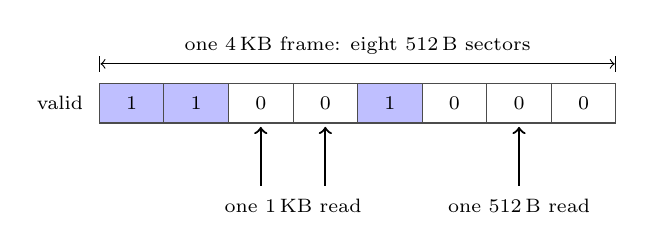
\begin{tikzpicture}[x=0.82cm,y=0.5cm,every node/.style={font=\scriptsize}]
\foreach \i/\v in {0/1,1/1,2/0,3/0,4/1,5/0,6/0,7/0}{
  \ifnum\v=1 \filldraw[fill=blue!25,draw=black!70] (\i,0) rectangle (\i+1,1);
  \else \draw[draw=black!70] (\i,0) rectangle (\i+1,1); \fi
  \node at (\i+.5,.5) {\v};
}
\node[anchor=east] at (-.1,.5) {valid};
\draw[|<->|] (0,1.5)--(8,1.5) node[midway,above] {one 4\,KB frame: eight 512\,B sectors};
\draw[thick,->] (2.5,-1.6)--(2.5,-.1);
\draw[thick,->] (3.5,-1.6)--(3.5,-.1);
\node at (3,-2.1) {one 1\,KB read};
\draw[thick,->] (6.5,-1.6)--(6.5,-.1);
\node at (6.5,-2.1) {one 512\,B read};
\end{tikzpicture}
\caption{Adaptive frame. Needed sectors 2, 3, and 6 cost two device operations, since each contiguous run is one read.}\label{fig:adaptive}
\end{figure}

\section{Methodology}
\subsection{Harness and baseline}
The harness is Python with NumPy; data files are real and are read with \texttt{pread}. \textbf{The baseline is a reconstruction.}
The original toy simulator was not available, so we re-implemented on-disk CSR, a second-chance clock cache, and warp-style coalescing from the BaM
paper~\cite{bam} and a written specification. Second-chance replacement differs from BaM's counter-only clock. Warps are simulated as groups of 32 list requests.

\subsection{Graphs}
Table~\ref{tab:graphs} summarises the inputs. \texttt{random} is a uniform directed graph. \texttt{powerlaw} is synthetic: truncated-Pareto out-degrees, with 80\% of
edges landing near the source at heavy-tailed ID distance and the rest on popular global targets. Parameters are ours and are not fitted to a real graph.
\texttt{web-Google} is a real web graph from SNAP~\cite{snapcommunity} using its numeric ID order; \texttt{web-Google-BFS} is the same graph relabelled by breadth-first
traversal, in the spirit of bandwidth-reducing orderings~\cite{cuthill,gorder}. All graphs are sorted and deduplicated.

\begin{table}[t]
\caption{Graphs. Raw size is 4 bytes per edge. ``Size'' is compressed relative to raw; ``Pad'' is added file size from padding.}\label{tab:graphs}
\small\setlength{\tabcolsep}{3.5pt}
\begin{tabular}{@{}lrrrrrr@{}}
\toprule
& & & \multicolumn{2}{c}{Bytes/edge} & & \\
\cmidrule(lr){4-5}
Graph & Nodes & Edges & Strad. & Pad. & Size & Pad \\
\midrule
\tblinput{generated/datasets.tex}
\bottomrule
\end{tabular}
\end{table}

\subsection{Workload and parameters}
Each run starts with a cold cache and executes 2,000 $k$-hop queries from uniformly random seeds, one batch per BFS level. Five query seeds
are used; synthetic graphs are fixed at generator seed 0. The default configuration is a cache of 2\% of raw graph size, depth 2, 4\,KB lines, $N=3$, and sorted frontiers. We vary one
factor at a time: cache size (0.1--50\%), depth (1--3), line size (512\,B--64\,KB), $N$ (0--99), and frontier order (sorted or shuffled).

\subsection{Metrics and device model}
We count storage bytes, misses, hits, coalesced accesses, and the size of every device read. Hit rate is hits per unique line probe. Confidence intervals are two-sided 95\% Student-$t$ intervals over paired per-seed
differences ($n=5$). Because reads come from the OS page cache, measured wall time contains no device cost and is dominated by Python
simulation overhead. We therefore \emph{model} storage time, summing a per-operation cost:
\begin{align}
  t_{\mathrm{NAND}}(s) &= \max\left(\frac{1}{750\,\mathrm{K}},\ \frac{s}{7\,\mathrm{GB/s}}\right),\\
  t_{\mathrm{Optane}}(s) &= \frac{1}{5.1\,\mathrm{M}} + \max(s-512,0)\,\frac{1/1.5\,\mathrm{M} - 1/5.1\,\mathrm{M}}{3584}.
\end{align}
Rates come from BaM's device table~\cite{bam} (980\,Pro: 700--800\,K read IOPS; P5800X: 5.1\,M at 512\,B, 1.5\,M at 4\,KB). The 7\,GB/s NAND transfer limit is
our assumption for PCIe Gen4 x4. This is a throughput model of one device, without queueing or latency.

Decode time is measured in two ways. \emph{Measured} decode is the in-run time, with one call per frontier batch. \emph{Bulk} decode applies a sequentially calibrated
rate to the edge count, excluding per-call overhead. The calibrated decoder runs at \nsMin--\nsMax\,ns/edge, with \usMin--\usMax\,$\mu$s for a 16-list batch. We report bulk decode where possible,
since it favours compression.

\subsection{Correctness and reproducibility}
A pytest suite of 423 cases compares every store with both load-all and an independent pure-Python BFS across multiple seeds, graphs, depths, cache sizes, and line sizes. Edge cases include
degree-0 nodes, reads past end of file, and a hub whose list exceeds the entire cache. An independent scalar decoder cross-checks the NumPy decoder. A differential test requires the new cache code in raw, full-line mode to reproduce
the baseline's counters exactly, so format comparisons are not artefacts of reimplementation. At runtime, a hash of every query result was compared with load-all for all 1,700 runs, with no mismatch.
Two complete benchmark executions produced identical bytes, misses, hits, and operation counts in all 340 summary rows. Timings are not deterministic: mean decode time for a configuration differed by up to 24\% between the runs.

\section{Results}
Table~\ref{tab:default} gives absolute results at the default point, and Table~\ref{tab:paired} gives paired changes against \store{Raw-4K}.

\begin{table*}[t]
\caption{Default point: cache 2\% of raw graph, depth 2, 4\,KB lines, $N=3$; means over five query seeds. Amp shown $\pm$ one standard deviation. NAND and Optane are modelled. \store{Raw-4K} decode is reported as 0 because its copy runs inside the baseline, untimed; \store{Adapt-R}'s value is that same copy.}\label{tab:default}
\small
\begin{tabular}{@{}lrrrrrrrrrr@{}}
\toprule
Store & Storage MB & Amp & Misses & Hit rate & Coalesced \% & Decode ms (measured) & Decode ms (bulk) & Wall s & NAND I/O ms & Optane I/O ms \\
\tblinput{generated/default.tex}
\bottomrule
\end{tabular}
\end{table*}

\begin{table}[t]
\caption{Change (\%) relative to \store{Raw-4K} at the default point, with paired 95\% CI ($n=5$). Negative is better.}\label{tab:paired}
\small\setlength{\tabcolsep}{2.5pt}
\begin{tabular}{@{}lrrrrr@{}}
\toprule
Store & Bytes & Misses & Dev.\ ops & NAND I/O & Optane I/O \\
\tblinput{generated/paired.tex}
\bottomrule
\end{tabular}
\end{table}

\subsection{H1: compression helps conditionally}
Without ID locality, compression barely helps. \texttt{random} and \texttt{web-Google} shrink to about 70\% of raw size, yet \store{Comp-S} reads only 1.3\% fewer bytes: under sparse cold access, each list
still costs about one line, whatever the line's density. Benefits appear when a line's additional lists are actually used. With locality, bytes and misses fall 15--20\%, and coalescing on \texttt{web-Google-BFS} rises from 28.5\% to 34.1\%.
Benefits also grow with cache size (Figure~\ref{fig:cache}), because a fixed byte budget holds more of the graph. At a 50\% cache, misses fall 31\% on \texttt{random} and \texttt{web-Google},
50\% on \texttt{powerlaw}, and 51\% on \texttt{web-Google-BFS}. H1 is supported for bytes and misses, with strongly conditional effect size.

Reordering matters as much as encoding. BFS relabelling alone reduces \store{Raw-4K} bytes by 36\% at the default point, more than compression achieves on the same graph in that configuration.
Padding has little effect: at most about one percentage point in bytes, at the cost of 0.2--4.4\% more file and 50\% more index RAM.

\begin{figure*}[t]
\centering
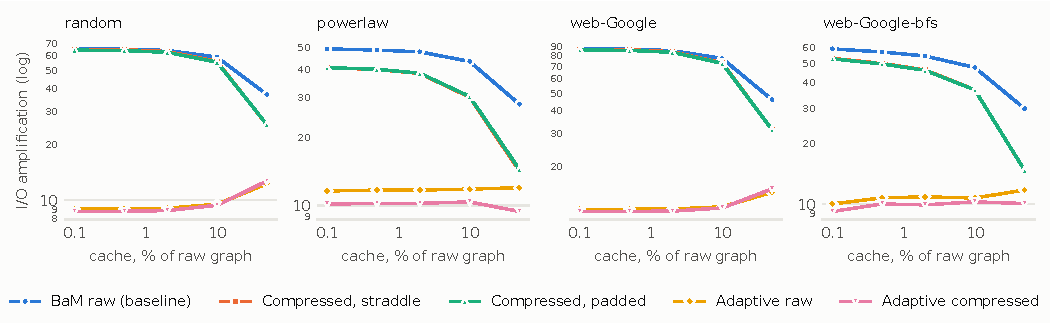
\includegraphics[width=\textwidth]{../results/amp_vs_cache.pdf}
\caption{I/O amplification against cache size (depth 2, 4\,KB lines; log scales). \store{Comp-S} and \store{Comp-P} nearly coincide. Adaptive lines sit far below at small caches, while compression closes the gap as the cache grows.}\label{fig:cache}
\end{figure*}

\subsection{RQ1: decode cost dominates compression's I/O savings}
Table~\ref{tab:breakeven} gives the decode speed at which \store{Comp-S} breaks even with \store{Raw-4K}. Our decoder is slower than break-even everywhere shown: the required speedup on NAND ranges from about 2$\times$ with
a large cache to 48$\times$ on \texttt{random} at the default point. Figure~\ref{fig:time} shows the resulting modelled total time. With bulk decode, plain compression beat the baseline only at 64\,KB lines (at most 6 of 280 paired runs per store), an impractical size at which raw reads are themselves
inflated. With measured decode, it never won. Encoding cost is small, at 0.3--1.1\,s per graph.

\begin{table}[t]
\caption{Break-even decode speed for \store{Comp-S} (ns/edge; higher is easier), and the speedup needed on NAND relative to our calibrated decoder.}\label{tab:breakeven}
\small\setlength{\tabcolsep}{3pt}
\begin{tabular}{@{}lrrrrrrr@{}}
\toprule
& & \multicolumn{3}{c}{Cache 2\%} & \multicolumn{3}{c}{Cache 50\%} \\
\cmidrule(lr){3-5}\cmidrule(lr){6-8}
Graph & Ours & NAND & Opt. & Need & NAND & Opt. & Need \\
\midrule
\tblinput{generated/breakeven.tex}
\bottomrule
\end{tabular}
\end{table}

\begin{figure*}[t]
\centering
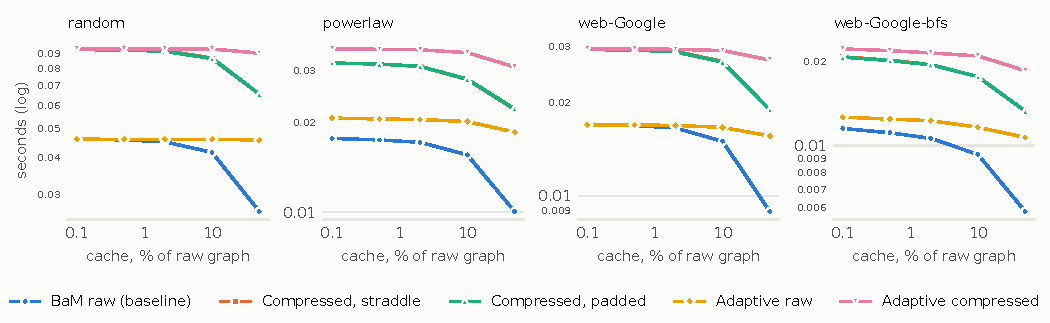
\includegraphics[width=\textwidth]{../results/time_vs_cache.pdf}
\caption{Modelled NAND I/O time plus bulk decode, in seconds (log scales). The raw baseline is fastest at every cache size; \store{Adapt-R} matches it only at small caches on graphs without locality.}\label{fig:time}
\end{figure*}

\subsection{H2 and RQ2: adaptive lines against smaller lines}
\store{Adapt-R} cuts bytes by 76--86\%, so H2 holds for bytes against 4\,KB lines. It fails for misses: \store{Adapt-R} incurs 1.6--11.5\% more, and hit rate drops sharply (0.126 to 0.050 on \texttt{web-Google-BFS}). Combining formats helps
only modestly: \store{Adapt-C} has about 5\% fewer misses on graphs with locality, still with more device operations, and reads 3--13\% fewer bytes than \store{Adapt-R}.

The stronger comparison is with a smaller fixed line (Table~\ref{tab:fixed}, Figure~\ref{fig:block}). Raw 512\,B lines give lower amplification than \store{Adapt-R} on all four graphs, 8.5--11.1 against 9.0--11.7. \store{Adapt-R}'s remaining advantages are 3--20\% fewer
device operations than 512\,B lines, and one eighth as many cache tags, which we did not include in the RAM accounting.

\begin{table}[t]
\caption{Adaptive 4\,KB lines against fixed raw lines at the default cache size. I/O in ms, modelled.}\label{tab:fixed}
\small\setlength{\tabcolsep}{3.5pt}
\begin{tabular}{@{}lrrrrrr@{}}
\toprule
Store & Amp & Hit rate & Misses & Dev.\ ops & NAND & Optane \\
\tblinput{generated/fixed.tex}
\bottomrule
\end{tabular}
\end{table}

\begin{figure*}[t]
\centering
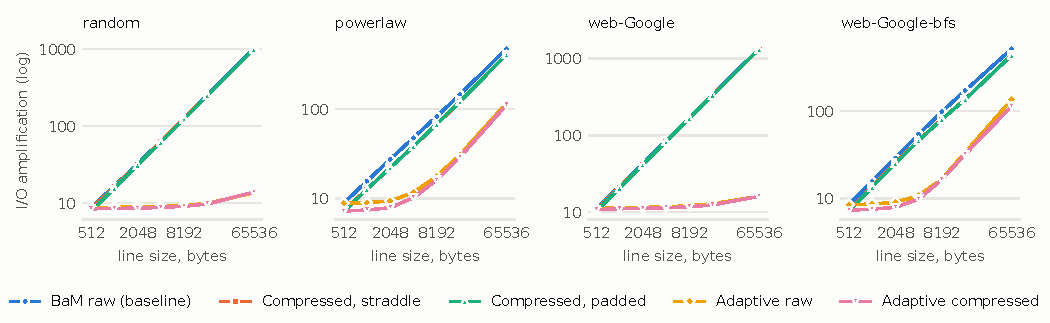
\includegraphics[width=\textwidth]{../results/amp_vs_block.pdf}
\caption{I/O amplification against line size (cache 2\%, depth 2; log scales). Sector granularity stays fixed at 512\,B for adaptive stores, so raw and adaptive curves converge at 512\,B.}\label{fig:block}
\end{figure*}

The upgrade rule did not earn its cost in bytes. Amplification falls monotonically as $N$ grows and is lowest when upgrades never fire (Figure~\ref{fig:threshold}). Upgrades also explain a counter-intuitive result: on \texttt{random}, \store{Adapt-R} amplification rises from 9.0 to 12.2 as the cache grows from
0.1\% to 50\%, because lines stay resident long enough to accumulate misses, taking upgrades from 4 to 3,768.

\begin{figure*}[t]
\centering
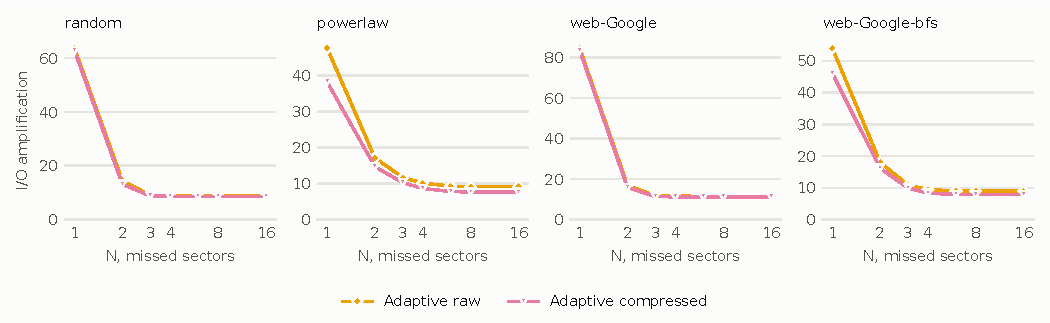
\includegraphics[width=\textwidth]{../results/amp_vs_threshold.pdf}
\caption{Adaptive amplification against upgrade threshold $N$. $N=1$ denotes a full-line fetch and 16 denotes upgrades disabled (measured with $N=99$).}\label{fig:threshold}
\end{figure*}

\subsection{RQ3: device sensitivity}
The time verdict on \store{Adapt-R} reverses with the device model. On Optane, modelled I/O falls 57--69\% since small reads are genuinely cheaper. On NAND, it rises 2--19\%, because a 512\,B read occupies the same IOPS slot as a 4\,KB read and adaptive issues more operations.
Across all sweeps, \store{Adapt-R} beat the baseline on total time in 260 of 280 Optane runs but in only 40 of 280 NAND runs, all of the latter at 16\,KB lines or larger.

\subsection{On-demand versus load-all}
Table~\ref{tab:depth} shows that deeper traversals favour load-all on this workload. At depth 3, load-all reads the fewest bytes on all four graphs. This reflects how much of the graph 2,000 queries reach. Load-all requires the entire graph in memory, the constraint BaM exists to
remove, so this is a statement about bytes only, not a recommendation.

\begin{table}[t]
\caption{Storage MB read by depth, with the smallest in bold. ``Need'' is raw MB requested.}\label{tab:depth}
\small\setlength{\tabcolsep}{3pt}
\begin{tabular}{@{}lrrrrrrr@{}}
\toprule
Graph & $k$ & Need & Load-all & Raw-4K & Comp-S & Adapt-R & Adapt-C \\
\midrule
\tblinput{generated/depth.tex}
\bottomrule
\end{tabular}
\end{table}

\section{Discussion}
Three practical implications follow. First, ordering should come before encoding: relabelling is free at query time and it benefits every format.
Second, sub-line fetching is most of the way achievable with a smaller fixed line, so a more complex adaptive scheme needs to justify itself through operation counts or tag overhead rather than bytes. Third, compression is worth revisiting only with a much faster decoder and
a cache that holds a meaningful fraction of the graph. SIMD integer decoders achieve very high throughput~\cite{lemire}, and such a decoder might reach the break-even range in Table~\ref{tab:breakeven}, but we did not measure one, and a GPU decoder would face its own constraints.

\section{Threats to Validity}
\paragraph{Internal validity.}
The baseline is a reconstruction and has not been compared with the original simulator. Its replacement policy differs from BaM's. Differential tests show that new and baseline cache code agree with each other, not that either
matches BaM. Decode times were taken with up to eight concurrent workers on 24 cores, and differed by up to 24\% between runs; we do not rely on small timing differences.

\paragraph{Construct validity.}
Storage time comes from a simple model, and RQ3's outcome depends on it. Real arrays, queueing, and PCIe limits could change the balance; link-bandwidth bottlenecks would favour adaptive fetching.
Hit rates are not directly comparable across formats, since stores probe different lines and adaptive partial hits count as misses. Tag and bitmap memory are not accounted for. Nothing here measures GPU throughput, contention, or latency, and a 4\,KB-formatted drive would preclude sub-4\,KB reads.

\paragraph{External validity.}
We used one real graph of about 5 million edges, smaller than the graphs BaM targets, and one instance of each synthetic graph. Our power-law locality parameters are unvalidated. The workload is uniform-seed $k$-hop traversal without concurrency; skewed query popularity could increase cache value and could help compression.
Sweeps vary one factor at a time, so interactions are largely untested, and the run counts reported above depend on which points were swept.

\section{Related Work}
BaM~\cite{bam} supplies the architecture studied here, and ActivePointers~\cite{activepointers} is earlier work on demand paging from GPUs. WebGraph~\cite{webgraph} established compression that exploits locality in web graphs, and Ligra+~\cite{ligraplus} showed that compressed graphs can be processed in parallel in memory; our work instead asks how compression interacts with a storage-backed
line cache. Fast integer decoding is studied by Lemire and Boytsov~\cite{lemire}. Cache compression has been explored for on-chip caches, for example Base-Delta-Immediate~\cite{bdi}. Sectored fetch dates to the System/360 Model~85~\cite{liptay}, and Footprint Cache~\cite{footprint} applies selective block fetching to die-stacked DRAM caches. Graph reordering is treated by Cuthill and McKee~\cite{cuthill} and by Gorder~\cite{gorder}.

\section{Conclusion}
Neither format is a straightforward replacement for raw 4\,KB lines. Compression reliably reduces bytes and misses, by an amount governed by locality and cache size, but our decoder gives back more time than the I/O saves. Adaptive lines greatly reduce bytes but raise misses in raw form, are matched by fixed 512\,B lines on bytes, and help time only on devices where small reads are cheap.
Future work should compare against the original baseline, evaluate a native decoder, test real devices and skewed workloads, include larger graphs such as soc-LiveJournal1, and account for metadata costs.

\section*{Data and Artifact Availability}
The code, per-seed results (\texttt{results/runs.csv}), and table generators accompany this paper in the project repository. \texttt{web-Google} is available from the SNAP collection. The benchmark ran on Linux with Python 3.14 and NumPy 2.5.4.

\begin{acks}
Generative AI (Claude Opus 5.5, Anthropic) was used to implement the harness, run the experiments, analyse results, and draft this manuscript. The author is responsible for reviewing and validating the work. No external funding was received.
\end{acks}

\bibliographystyle{ACM-Reference-Format}
\bibliography{refs}
\end{document}
